\documentclass[1p]{elsarticle_modified}
%\bibliographystyle{elsarticle-num}

%\usepackage[colorlinks]{hyperref}
%\usepackage{abbrmath_seonhwa} %\Abb, \Ascr, \Acal ,\Abf, \Afrak
\usepackage{amsfonts}
\usepackage{amssymb}
\usepackage{amsmath}
\usepackage{amsthm}
\usepackage{scalefnt}
\usepackage{amsbsy}
\usepackage{kotex}
\usepackage{caption}
\usepackage{subfig}
\usepackage{color}
\usepackage{graphicx}
\usepackage{xcolor} %% white, black, red, green, blue, cyan, magenta, yellow
\usepackage{float}
\usepackage{setspace}
\usepackage{hyperref}

\usepackage{tikz}
\usetikzlibrary{arrows}

\usepackage{multirow}
\usepackage{array} % fixed length table
\usepackage{hhline}

%%%%%%%%%%%%%%%%%%%%%
\makeatletter
\renewcommand*\env@matrix[1][\arraystretch]{%
	\edef\arraystretch{#1}%
	\hskip -\arraycolsep
	\let\@ifnextchar\new@ifnextchar
	\array{*\c@MaxMatrixCols c}}
\makeatother %https://tex.stackexchange.com/questions/14071/how-can-i-increase-the-line-spacing-in-a-matrix
%%%%%%%%%%%%%%%

\usepackage[normalem]{ulem}

\newcommand{\msout}[1]{\ifmmode\text{\sout{\ensuremath{#1}}}\else\sout{#1}\fi}
%SOURCE: \msout is \stkout macro in https://tex.stackexchange.com/questions/20609/strikeout-in-math-mode

\newcommand{\cancel}[1]{
	\ifmmode
	{\color{red}\msout{#1}}
	\else
	{\color{red}\sout{#1}}
	\fi
}

\newcommand{\add}[1]{
	{\color{blue}\uwave{#1}}
}

\newcommand{\replace}[2]{
	\ifmmode
	{\color{red}\msout{#1}}{\color{blue}\uwave{#2}}
	\else
	{\color{red}\sout{#1}}{\color{blue}\uwave{#2}}
	\fi
}

\newcommand{\Sol}{\mathcal{S}} %segment
\newcommand{\D}{D} %diagram
\newcommand{\A}{\mathcal{A}} %arc


%%%%%%%%%%%%%%%%%%%%%%%%%%%%%5 test

\def\sl{\operatorname{\textup{SL}}(2,\Cbb)}
\def\psl{\operatorname{\textup{PSL}}(2,\Cbb)}
\def\quan{\mkern 1mu \triangleright \mkern 1mu}

\theoremstyle{definition}
\newtheorem{thm}{Theorem}[section]
\newtheorem{prop}[thm]{Proposition}
\newtheorem{lem}[thm]{Lemma}
\newtheorem{ques}[thm]{Question}
\newtheorem{cor}[thm]{Corollary}
\newtheorem{defn}[thm]{Definition}
\newtheorem{exam}[thm]{Example}
\newtheorem{rmk}[thm]{Remark}
\newtheorem{alg}[thm]{Algorithm}

\newcommand{\I}{\sqrt{-1}}
\begin{document}

%\begin{frontmatter}
%
%\title{Boundary parabolic representations of knots up to 8 crossings}
%
%%% Group authors per affiliation:
%\author{Yunhi Cho} 
%\address{Department of Mathematics, University of Seoul, Seoul, Korea}
%\ead{yhcho@uos.ac.kr}
%
%
%\author{Seonhwa Kim} %\fnref{s_kim}}
%\address{Center for Geometry and Physics, Institute for Basic Science, Pohang, 37673, Korea}
%\ead{ryeona17@ibs.re.kr}
%
%\author{Hyuk Kim}
%\address{Department of Mathematical Sciences, Seoul National University, Seoul 08826, Korea}
%\ead{hyukkim@snu.ac.kr}
%
%\author{Seokbeom Yoon}
%\address{Department of Mathematical Sciences, Seoul National University, Seoul, 08826,  Korea}
%\ead{sbyoon15@snu.ac.kr}
%
%\begin{abstract}
%We find all boundary parabolic representation of knots up to 8 crossings.
%
%\end{abstract}
%\begin{keyword}
%    \MSC[2010] 57M25 
%\end{keyword}
%
%\end{frontmatter}

%\linenumbers
%\tableofcontents
%
\newcommand\colored[1]{\textcolor{white}{\rule[-0.35ex]{0.8em}{1.4ex}}\kern-0.8em\color{red} #1}%
%\newcommand\colored[1]{\textcolor{white}{ #1}\kern-2.17ex	\textcolor{white}{ #1}\kern-1.81ex	\textcolor{white}{ #1}\kern-2.15ex\color{red}#1	}

{\Large $\underline{12a_{0516}~(K12a_{0516})}$}

\setlength{\tabcolsep}{10pt}
\renewcommand{\arraystretch}{1.6}
\vspace{1cm}\begin{tabular}{m{100pt}>{\centering\arraybackslash}m{274pt}}
\multirow{5}{120pt}{
	\centering
	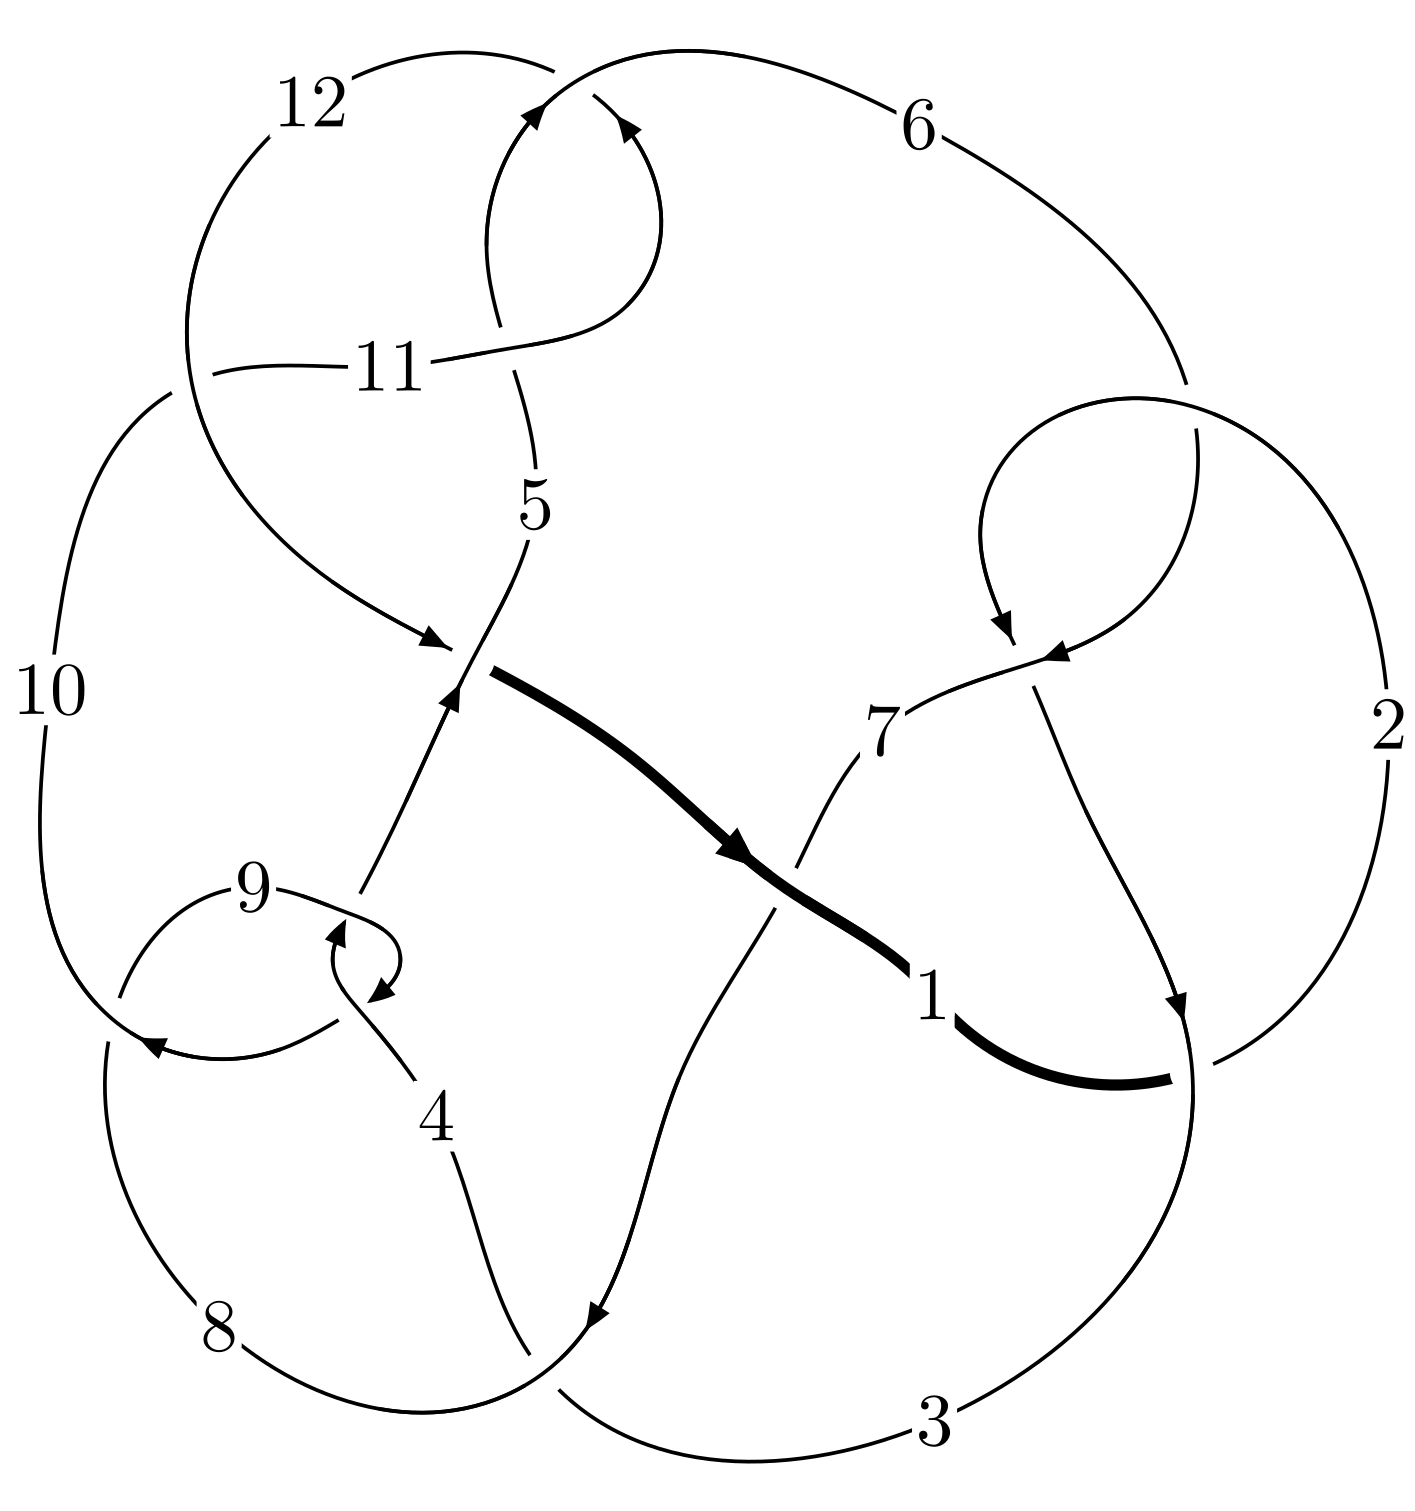
\includegraphics[width=112pt]{../../../GIT/diagram.site/Diagrams/png/1317_12a_0516.png}\\
\ \ \ A knot diagram\footnotemark}&
\allowdisplaybreaks
\textbf{Linearized knot diagam} \\
\cline{2-2}
 &
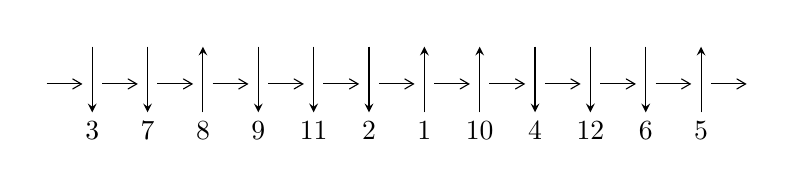
\begin{tikzpicture}[x=20pt, y=17pt]
	% nodes
	\node (C0) at (0, 0) {};
	\node (C1) at (1, 0) {};
	\node (C1U) at (1, +1) {};
	\node (C1D) at (1, -1) {3};

	\node (C2) at (2, 0) {};
	\node (C2U) at (2, +1) {};
	\node (C2D) at (2, -1) {7};

	\node (C3) at (3, 0) {};
	\node (C3U) at (3, +1) {};
	\node (C3D) at (3, -1) {8};

	\node (C4) at (4, 0) {};
	\node (C4U) at (4, +1) {};
	\node (C4D) at (4, -1) {9};

	\node (C5) at (5, 0) {};
	\node (C5U) at (5, +1) {};
	\node (C5D) at (5, -1) {11};

	\node (C6) at (6, 0) {};
	\node (C6U) at (6, +1) {};
	\node (C6D) at (6, -1) {2};

	\node (C7) at (7, 0) {};
	\node (C7U) at (7, +1) {};
	\node (C7D) at (7, -1) {1};

	\node (C8) at (8, 0) {};
	\node (C8U) at (8, +1) {};
	\node (C8D) at (8, -1) {10};

	\node (C9) at (9, 0) {};
	\node (C9U) at (9, +1) {};
	\node (C9D) at (9, -1) {4};

	\node (C10) at (10, 0) {};
	\node (C10U) at (10, +1) {};
	\node (C10D) at (10, -1) {12};

	\node (C11) at (11, 0) {};
	\node (C11U) at (11, +1) {};
	\node (C11D) at (11, -1) {6};

	\node (C12) at (12, 0) {};
	\node (C12U) at (12, +1) {};
	\node (C12D) at (12, -1) {5};
	\node (C13) at (13, 0) {};

	% arrows
	\draw[->,>={angle 60}]
	(C0) edge (C1) (C1) edge (C2) (C2) edge (C3) (C3) edge (C4) (C4) edge (C5) (C5) edge (C6) (C6) edge (C7) (C7) edge (C8) (C8) edge (C9) (C9) edge (C10) (C10) edge (C11) (C11) edge (C12) (C12) edge (C13) ;	\draw[->,>=stealth]
	(C1U) edge (C1D) (C2U) edge (C2D) (C3D) edge (C3U) (C4U) edge (C4D) (C5U) edge (C5D) (C6U) edge (C6D) (C7D) edge (C7U) (C8D) edge (C8U) (C9U) edge (C9D) (C10U) edge (C10D) (C11U) edge (C11D) (C12D) edge (C12U) ;
	\end{tikzpicture} \\
\hhline{~~} \\& 
\textbf{Solving Sequence} \\ \cline{2-2} 
 &
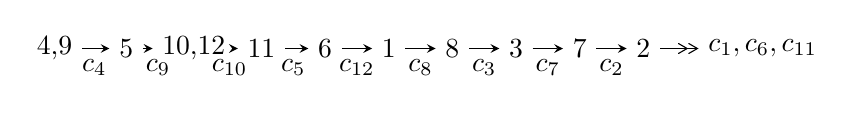
\begin{tikzpicture}[x=23pt, y=7pt]
	% node
	\node (A0) at (-1/8, 0) {4,9};
	\node (A1) at (1, 0) {5};
	\node (A2) at (33/16, 0) {10,12};
	\node (A3) at (25/8, 0) {11};
	\node (A4) at (33/8, 0) {6};
	\node (A5) at (41/8, 0) {1};
	\node (A6) at (49/8, 0) {8};
	\node (A7) at (57/8, 0) {3};
	\node (A8) at (65/8, 0) {7};
	\node (A9) at (73/8, 0) {2};
	\node (C1) at (1/2, -1) {$c_{4}$};
	\node (C2) at (3/2, -1) {$c_{9}$};
	\node (C3) at (21/8, -1) {$c_{10}$};
	\node (C4) at (29/8, -1) {$c_{5}$};
	\node (C5) at (37/8, -1) {$c_{12}$};
	\node (C6) at (45/8, -1) {$c_{8}$};
	\node (C7) at (53/8, -1) {$c_{3}$};
	\node (C8) at (61/8, -1) {$c_{7}$};
	\node (C9) at (69/8, -1) {$c_{2}$};
	\node (A10) at (11, 0) {$c_{1},c_{6},c_{11}$};

	% edge
	\draw[->,>=stealth]	
	(A0) edge (A1) (A1) edge (A2) (A2) edge (A3) (A3) edge (A4) (A4) edge (A5) (A5) edge (A6) (A6) edge (A7) (A7) edge (A8) (A8) edge (A9) ;
	\draw[->>,>={angle 60}]	
	(A9) edge (A10);
\end{tikzpicture} \\ 

\end{tabular} \\

\footnotetext{
The image of knot diagram is generated by the software ``\textbf{Draw programme}" developed by Andrew Bartholomew(\url{http://www.layer8.co.uk/maths/draw/index.htm\#Running-draw}), where we modified some parts for our purpose(\url{https://github.com/CATsTAILs/LinksPainter}).
}\phantom \\ \newline 
\centering \textbf{Ideals for irreducible components\footnotemark of $X_{\text{par}}$} 
 
\begin{align*}
I^u_{1}&=\langle 
-3 u^{26}+19 u^{25}+\cdots+4 b+2,\;11 u^{26}-57 u^{25}+\cdots+8 a-62,\;u^{27}-5 u^{26}+\cdots-12 u+4\rangle \\
I^u_{2}&=\langle 
153018 u^{43} a+172574 u^{43}+\cdots+267932 a+346978,\;-5 u^{43} a-8 u^{42} a+\cdots-7 a-8,\\
\phantom{I^u_{2}}&\phantom{= \langle  }u^{44}+2 u^{43}+\cdots+2 u+1\rangle \\
I^u_{3}&=\langle 
- a u+b+a,\;a^2- a+1,\;u^2+1\rangle \\
I^u_{4}&=\langle 
a u+b+a- u,\;a^2- a+1,\;u^2+1\rangle \\
\\
\end{align*}
\raggedright * 4 irreducible components of $\dim_{\mathbb{C}}=0$, with total 123 representations.\\
\footnotetext{All coefficients of polynomials are rational numbers. But the coefficients are sometimes approximated in decimal forms when there is not enough margin.}
\newpage
\renewcommand{\arraystretch}{1}
\centering \section*{I. $I^u_{1}= \langle -3 u^{26}+19 u^{25}+\cdots+4 b+2,\;11 u^{26}-57 u^{25}+\cdots+8 a-62,\;u^{27}-5 u^{26}+\cdots-12 u+4 \rangle$}
\flushleft \textbf{(i) Arc colorings}\\
\begin{tabular}{m{7pt} m{180pt} m{7pt} m{180pt} }
\flushright $a_{4}=$&$\begin{pmatrix}1\\0\end{pmatrix}$ \\
\flushright $a_{9}=$&$\begin{pmatrix}0\\u\end{pmatrix}$ \\
\flushright $a_{5}=$&$\begin{pmatrix}1\\u^2\end{pmatrix}$ \\
\flushright $a_{10}=$&$\begin{pmatrix}- u\\u\end{pmatrix}$ \\
\flushright $a_{12}=$&$\begin{pmatrix}-1.37500 u^{26}+7.12500 u^{25}+\cdots-19.8750 u+7.75000\\\frac{3}{4} u^{26}-\frac{19}{4} u^{25}+\cdots+\frac{33}{4} u-\frac{1}{2}\end{pmatrix}$ \\
\flushright $a_{11}=$&$\begin{pmatrix}-\frac{3}{8} u^{26}+\frac{13}{8} u^{25}+\cdots-\frac{35}{8} u+\frac{5}{4}\\\frac{1}{4} u^{26}-\frac{5}{4} u^{25}+\cdots+\frac{11}{4} u-\frac{1}{2}\end{pmatrix}$ \\
\flushright $a_{6}=$&$\begin{pmatrix}\frac{1}{8} u^{26}+\frac{1}{8} u^{25}+\cdots-\frac{67}{8} u+\frac{27}{4}\\-\frac{1}{4} u^{26}+\frac{1}{4} u^{25}+\cdots+\frac{35}{4} u-\frac{11}{2}\end{pmatrix}$ \\
\flushright $a_{1}=$&$\begin{pmatrix}-1.62500 u^{26}+8.37500 u^{25}+\cdots-20.1250 u+8.25000\\\frac{7}{4} u^{26}-\frac{29}{4} u^{25}+\cdots+\frac{37}{4} u-\frac{1}{2}\end{pmatrix}$ \\
\flushright $a_{8}=$&$\begin{pmatrix}- u^3\\u^3+u\end{pmatrix}$ \\
\flushright $a_{3}=$&$\begin{pmatrix}- u^6- u^4+1\\u^6+2 u^4+u^2\end{pmatrix}$ \\
\flushright $a_{7}=$&$\begin{pmatrix}-\frac{1}{8} u^{26}+\frac{3}{8} u^{25}+\cdots-\frac{1}{8} u-\frac{1}{4}\\-\frac{1}{4} u^{26}+\frac{5}{4} u^{25}+\cdots-\frac{9}{4} u+\frac{3}{2}\end{pmatrix}$ \\
\flushright $a_{2}=$&$\begin{pmatrix}\frac{1}{8} u^{26}-\frac{23}{8} u^{25}+\cdots+\frac{129}{8} u-\frac{25}{4}\\\frac{3}{4} u^{26}-\frac{1}{4} u^{25}+\cdots-\frac{7}{4} u-\frac{5}{2}\end{pmatrix}$\\&\end{tabular}
\flushleft \textbf{(ii) Obstruction class $= -1$}\\~\\
\flushleft \textbf{(iii) Cusp Shapes $= -3 u^{25}+11 u^{24}-41 u^{23}+94 u^{22}-201 u^{21}+350 u^{20}-555 u^{19}+811 u^{18}-1060 u^{17}+1348 u^{16}-1524 u^{15}+1683 u^{14}-1695 u^{13}+1624 u^{12}-1489 u^{11}+1249 u^{10}-1017 u^9+745 u^8-495 u^7+304 u^6-145 u^5+54 u^4-7 u^3-21 u^2+20 u-6$}\\~\\
\newpage\renewcommand{\arraystretch}{1}
\flushleft \textbf{(iv) u-Polynomials at the component}\newline \\
\begin{tabular}{m{50pt}|m{274pt}}
Crossings & \hspace{64pt}u-Polynomials at each crossing \\
\hline $$\begin{aligned}c_{1},c_{10}\end{aligned}$$&$\begin{aligned}
&u^{27}+14 u^{26}+\cdots+4 u+1
\end{aligned}$\\
\hline $$\begin{aligned}c_{2},c_{5},c_{6}\\c_{11}\end{aligned}$$&$\begin{aligned}
&u^{27}-7 u^{25}+\cdots-2 u^2+1
\end{aligned}$\\
\hline $$\begin{aligned}c_{3}\end{aligned}$$&$\begin{aligned}
&u^{27}+5 u^{26}+\cdots-320 u^2+64
\end{aligned}$\\
\hline $$\begin{aligned}c_{4},c_{9}\end{aligned}$$&$\begin{aligned}
&u^{27}-5 u^{26}+\cdots-12 u+4
\end{aligned}$\\
\hline $$\begin{aligned}c_{7},c_{12}\end{aligned}$$&$\begin{aligned}
&u^{27}+5 u^{25}+\cdots-2 u+3
\end{aligned}$\\
\hline $$\begin{aligned}c_{8}\end{aligned}$$&$\begin{aligned}
&u^{27}-15 u^{26}+\cdots+56 u+16
\end{aligned}$\\
\hline
\end{tabular}\\~\\
\newpage\renewcommand{\arraystretch}{1}
\flushleft \textbf{(v) Riley Polynomials at the component}\newline \\
\begin{tabular}{m{50pt}|m{274pt}}
Crossings & \hspace{64pt}Riley Polynomials at each crossing \\
\hline $$\begin{aligned}c_{1},c_{10}\end{aligned}$$&$\begin{aligned}
&y^{27}+2 y^{26}+\cdots+8 y-1
\end{aligned}$\\
\hline $$\begin{aligned}c_{2},c_{5},c_{6}\\c_{11}\end{aligned}$$&$\begin{aligned}
&y^{27}-14 y^{26}+\cdots+4 y-1
\end{aligned}$\\
\hline $$\begin{aligned}c_{3}\end{aligned}$$&$\begin{aligned}
&y^{27}-13 y^{26}+\cdots+40960 y-4096
\end{aligned}$\\
\hline $$\begin{aligned}c_{4},c_{9}\end{aligned}$$&$\begin{aligned}
&y^{27}+15 y^{26}+\cdots+56 y-16
\end{aligned}$\\
\hline $$\begin{aligned}c_{7},c_{12}\end{aligned}$$&$\begin{aligned}
&y^{27}+10 y^{26}+\cdots-20 y-9
\end{aligned}$\\
\hline $$\begin{aligned}c_{8}\end{aligned}$$&$\begin{aligned}
&y^{27}-5 y^{26}+\cdots+8480 y-256
\end{aligned}$\\
\hline
\end{tabular}\\~\\
\newpage\flushleft \textbf{(vi) Complex Volumes and Cusp Shapes}
$$\begin{array}{c|c|c}  
\text{Solutions to }I^u_{1}& \I (\text{vol} + \sqrt{-1}CS) & \text{Cusp shape}\\
 \hline 
\begin{aligned}
u &= -0.730663 + 0.630842 I \\
a &= -1.15948 + 1.36199 I \\
b &= \phantom{-}1.380630 + 0.132263 I\end{aligned}
 & -6.78998 - 5.25258 I & -11.87823 + 4.55008 I \\ \hline\begin{aligned}
u &= -0.730663 - 0.630842 I \\
a &= -1.15948 - 1.36199 I \\
b &= \phantom{-}1.380630 - 0.132263 I\end{aligned}
 & -6.78998 + 5.25258 I & -11.87823 - 4.55008 I \\ \hline\begin{aligned}
u &= -0.496338 + 0.799160 I \\
a &= \phantom{-}0.491347 - 1.120530 I \\
b &= -0.828650 + 0.873109 I\end{aligned}
 & -0.34967 + 2.03126 I & -2.38031 - 3.61940 I \\ \hline\begin{aligned}
u &= -0.496338 - 0.799160 I \\
a &= \phantom{-}0.491347 + 1.120530 I \\
b &= -0.828650 - 0.873109 I\end{aligned}
 & -0.34967 - 2.03126 I & -2.38031 + 3.61940 I \\ \hline\begin{aligned}
u &= \phantom{-}0.893419 + 0.201765 I \\
a &= \phantom{-}0.47034 + 1.60999 I \\
b &= -1.108620 - 0.003316 I\end{aligned}
 & -1.56275 + 12.48900 I & -7.13823 - 8.79182 I \\ \hline\begin{aligned}
u &= \phantom{-}0.893419 - 0.201765 I \\
a &= \phantom{-}0.47034 - 1.60999 I \\
b &= -1.108620 + 0.003316 I\end{aligned}
 & -1.56275 - 12.48900 I & -7.13823 + 8.79182 I \\ \hline\begin{aligned}
u &= -0.178235 + 1.084250 I \\
a &= -0.213163 - 0.502908 I \\
b &= \phantom{-}0.659574 + 0.702653 I\end{aligned}
 & \phantom{-}1.94164 + 2.20192 I & -0.56198 - 2.41318 I \\ \hline\begin{aligned}
u &= -0.178235 - 1.084250 I \\
a &= -0.213163 + 0.502908 I \\
b &= \phantom{-}0.659574 - 0.702653 I\end{aligned}
 & \phantom{-}1.94164 - 2.20192 I & -0.56198 + 2.41318 I \\ \hline\begin{aligned}
u &= -0.664783 + 0.914963 I \\
a &= -0.39003 + 1.65011 I \\
b &= \phantom{-}1.72361 - 1.44912 I\end{aligned}
 & -5.96942 + 10.50660 I & -9.69062 - 10.08606 I \\ \hline\begin{aligned}
u &= -0.664783 - 0.914963 I \\
a &= -0.39003 - 1.65011 I \\
b &= \phantom{-}1.72361 + 1.44912 I\end{aligned}
 & -5.96942 - 10.50660 I & -9.69062 + 10.08606 I\\
 \hline 
 \end{array}$$\newpage$$\begin{array}{c|c|c}  
\text{Solutions to }I^u_{1}& \I (\text{vol} + \sqrt{-1}CS) & \text{Cusp shape}\\
 \hline 
\begin{aligned}
u &= \phantom{-}0.728836 + 0.456068 I \\
a &= -0.664583 + 0.952860 I \\
b &= -0.840437 - 0.847346 I\end{aligned}
 & -5.99030 - 2.50292 I & -13.30644 + 3.87606 I \\ \hline\begin{aligned}
u &= \phantom{-}0.728836 - 0.456068 I \\
a &= -0.664583 - 0.952860 I \\
b &= -0.840437 + 0.847346 I\end{aligned}
 & -5.99030 + 2.50292 I & -13.30644 - 3.87606 I \\ \hline\begin{aligned}
u &= \phantom{-}0.799916 + 0.147492 I \\
a &= -0.553123 - 0.901764 I \\
b &= \phantom{-}0.879493 + 0.088034 I\end{aligned}
 & \phantom{-}2.62362 + 2.33182 I & -0.926585 - 0.602280 I \\ \hline\begin{aligned}
u &= \phantom{-}0.799916 - 0.147492 I \\
a &= -0.553123 + 0.901764 I \\
b &= \phantom{-}0.879493 - 0.088034 I\end{aligned}
 & \phantom{-}2.62362 - 2.33182 I & -0.926585 + 0.602280 I \\ \hline\begin{aligned}
u &= \phantom{-}0.563387 + 1.046610 I \\
a &= \phantom{-}1.253280 + 0.526603 I \\
b &= -1.42614 + 0.54904 I\end{aligned}
 & -4.25210 - 2.40888 I & -10.75070 + 1.81073 I \\ \hline\begin{aligned}
u &= \phantom{-}0.563387 - 1.046610 I \\
a &= \phantom{-}1.253280 - 0.526603 I \\
b &= -1.42614 - 0.54904 I\end{aligned}
 & -4.25210 + 2.40888 I & -10.75070 - 1.81073 I \\ \hline\begin{aligned}
u &= \phantom{-}0.021698 + 1.237970 I \\
a &= \phantom{-}0.353870 + 0.098440 I \\
b &= -0.986014 + 0.581923 I\end{aligned}
 & -0.30811 - 4.23523 I & -8.52197 + 5.94232 I \\ \hline\begin{aligned}
u &= \phantom{-}0.021698 - 1.237970 I \\
a &= \phantom{-}0.353870 - 0.098440 I \\
b &= -0.986014 - 0.581923 I\end{aligned}
 & -0.30811 + 4.23523 I & -8.52197 - 5.94232 I \\ \hline\begin{aligned}
u &= \phantom{-}0.371922 + 1.216990 I \\
a &= -0.047378 - 0.727973 I \\
b &= -0.420071 + 0.350884 I\end{aligned}
 & \phantom{-}6.71645 - 1.62939 I & \phantom{-}3.63674 + 2.67627 I \\ \hline\begin{aligned}
u &= \phantom{-}0.371922 - 1.216990 I \\
a &= -0.047378 + 0.727973 I \\
b &= -0.420071 - 0.350884 I\end{aligned}
 & \phantom{-}6.71645 + 1.62939 I & \phantom{-}3.63674 - 2.67627 I\\
 \hline 
 \end{array}$$\newpage$$\begin{array}{c|c|c}  
\text{Solutions to }I^u_{1}& \I (\text{vol} + \sqrt{-1}CS) & \text{Cusp shape}\\
 \hline 
\begin{aligned}
u &= \phantom{-}0.517374 + 1.188310 I \\
a &= -0.98424 - 1.30505 I \\
b &= \phantom{-}1.59567 + 1.17935 I\end{aligned}
 & \phantom{-}5.67800 - 7.17879 I & \phantom{-}1.95902 + 3.78339 I \\ \hline\begin{aligned}
u &= \phantom{-}0.517374 - 1.188310 I \\
a &= -0.98424 + 1.30505 I \\
b &= \phantom{-}1.59567 - 1.17935 I\end{aligned}
 & \phantom{-}5.67800 + 7.17879 I & \phantom{-}1.95902 - 3.78339 I \\ \hline\begin{aligned}
u &= \phantom{-}0.322363 + 1.283180 I \\
a &= -0.258472 + 0.363453 I \\
b &= \phantom{-}1.027060 + 0.465180 I\end{aligned}
 & \phantom{-}3.19039 + 8.39996 I & -2.59631 - 7.43442 I \\ \hline\begin{aligned}
u &= \phantom{-}0.322363 - 1.283180 I \\
a &= -0.258472 - 0.363453 I \\
b &= \phantom{-}1.027060 - 0.465180 I\end{aligned}
 & \phantom{-}3.19039 - 8.39996 I & -2.59631 + 7.43442 I \\ \hline\begin{aligned}
u &= \phantom{-}0.559888 + 1.210030 I \\
a &= \phantom{-}1.36303 + 1.45255 I \\
b &= -2.57082 - 1.28259 I\end{aligned}
 & \phantom{-}1.4727 - 17.7774 I & -3.91820 + 11.76326 I \\ \hline\begin{aligned}
u &= \phantom{-}0.559888 - 1.210030 I \\
a &= \phantom{-}1.36303 - 1.45255 I \\
b &= -2.57082 + 1.28259 I\end{aligned}
 & \phantom{-}1.4727 + 17.7774 I & -3.91820 - 11.76326 I \\ \hline\begin{aligned}
u &= -0.417568\phantom{ +0.000000I} \\
a &= \phantom{-}1.17723\phantom{ +0.000000I} \\
b &= -0.170545\phantom{ +0.000000I}\end{aligned}
 & -1.02561\phantom{ +0.000000I} & -9.85230\phantom{ +0.000000I}\\
 \hline 
 \end{array}$$\newpage\newpage\renewcommand{\arraystretch}{1}
\centering \section*{II. $I^u_{2}= \langle 1.53\times10^{5} a u^{43}+1.73\times10^{5} u^{43}+\cdots+2.68\times10^{5} a+3.47\times10^{5},\;-5 u^{43} a-8 u^{42} a+\cdots-7 a-8,\;u^{44}+2 u^{43}+\cdots+2 u+1 \rangle$}
\flushleft \textbf{(i) Arc colorings}\\
\begin{tabular}{m{7pt} m{180pt} m{7pt} m{180pt} }
\flushright $a_{4}=$&$\begin{pmatrix}1\\0\end{pmatrix}$ \\
\flushright $a_{9}=$&$\begin{pmatrix}0\\u\end{pmatrix}$ \\
\flushright $a_{5}=$&$\begin{pmatrix}1\\u^2\end{pmatrix}$ \\
\flushright $a_{10}=$&$\begin{pmatrix}- u\\u\end{pmatrix}$ \\
\flushright $a_{12}=$&$\begin{pmatrix}a\\-0.671774 a u^{43}-0.757628 u^{43}+\cdots-1.17627 a-1.52329\end{pmatrix}$ \\
\flushright $a_{11}=$&$\begin{pmatrix}0.0879130 a u^{43}-1.35545 u^{43}+\cdots+1.75763 a-1.80612\\-0.0707343 a u^{43}-1.51109 u^{43}+\cdots-0.630357 a-1.70508\end{pmatrix}$ \\
\flushright $a_{6}=$&$\begin{pmatrix}1.17627 a u^{43}+1.52329 u^{43}+\cdots+1.06336 a+1.87686\\- a u\end{pmatrix}$ \\
\flushright $a_{1}=$&$\begin{pmatrix}-0.671774 a u^{43}-0.757628 u^{43}+\cdots-0.176265 a-1.52329\\-0.887094 a u^{43}+0.646425 u^{43}+\cdots-1.55887 a-1.11120\end{pmatrix}$ \\
\flushright $a_{8}=$&$\begin{pmatrix}- u^3\\u^3+u\end{pmatrix}$ \\
\flushright $a_{3}=$&$\begin{pmatrix}- u^6- u^4+1\\u^6+2 u^4+u^2\end{pmatrix}$ \\
\flushright $a_{7}=$&$\begin{pmatrix}0.757628 a u^{43}-1.80612 u^{43}+\cdots+1.52329 a-3.62675\\-1.40405 a u^{43}+0.130050 u^{43}+\cdots-0.412087 a-1.35545\end{pmatrix}$ \\
\flushright $a_{2}=$&$\begin{pmatrix}-0.337208 a u^{43}-1.77370 u^{43}+\cdots+0.402077 a-0.183860\\-0.671774 a u^{43}+1.74237 u^{43}+\cdots-1.17627 a-1.02329\end{pmatrix}$\\&\end{tabular}
\flushleft \textbf{(ii) Obstruction class $= -1$}\\~\\
\flushleft \textbf{(iii) Cusp Shapes $= -8 u^{42}-14 u^{41}+\cdots-10 u-8$}\\~\\
\newpage\renewcommand{\arraystretch}{1}
\flushleft \textbf{(iv) u-Polynomials at the component}\newline \\
\begin{tabular}{m{50pt}|m{274pt}}
Crossings & \hspace{64pt}u-Polynomials at each crossing \\
\hline $$\begin{aligned}c_{1},c_{10}\end{aligned}$$&$\begin{aligned}
&u^{88}+39 u^{87}+\cdots+18 u+1
\end{aligned}$\\
\hline $$\begin{aligned}c_{2},c_{5},c_{6}\\c_{11}\end{aligned}$$&$\begin{aligned}
&u^{88}- u^{87}+\cdots-6 u+1
\end{aligned}$\\
\hline $$\begin{aligned}c_{3}\end{aligned}$$&$\begin{aligned}
&(u^{44}-2 u^{43}+\cdots-16 u+4)^{2}
\end{aligned}$\\
\hline $$\begin{aligned}c_{4},c_{9}\end{aligned}$$&$\begin{aligned}
&(u^{44}+2 u^{43}+\cdots+2 u+1)^{2}
\end{aligned}$\\
\hline $$\begin{aligned}c_{7},c_{12}\end{aligned}$$&$\begin{aligned}
&u^{88}-3 u^{87}+\cdots-138 u+33
\end{aligned}$\\
\hline $$\begin{aligned}c_{8}\end{aligned}$$&$\begin{aligned}
&(u^{44}-24 u^{43}+\cdots-4 u+1)^{2}
\end{aligned}$\\
\hline
\end{tabular}\\~\\
\newpage\renewcommand{\arraystretch}{1}
\flushleft \textbf{(v) Riley Polynomials at the component}\newline \\
\begin{tabular}{m{50pt}|m{274pt}}
Crossings & \hspace{64pt}Riley Polynomials at each crossing \\
\hline $$\begin{aligned}c_{1},c_{10}\end{aligned}$$&$\begin{aligned}
&y^{88}+21 y^{87}+\cdots+238 y+1
\end{aligned}$\\
\hline $$\begin{aligned}c_{2},c_{5},c_{6}\\c_{11}\end{aligned}$$&$\begin{aligned}
&y^{88}-39 y^{87}+\cdots-18 y+1
\end{aligned}$\\
\hline $$\begin{aligned}c_{3}\end{aligned}$$&$\begin{aligned}
&(y^{44}-26 y^{43}+\cdots-232 y+16)^{2}
\end{aligned}$\\
\hline $$\begin{aligned}c_{4},c_{9}\end{aligned}$$&$\begin{aligned}
&(y^{44}+24 y^{43}+\cdots+4 y+1)^{2}
\end{aligned}$\\
\hline $$\begin{aligned}c_{7},c_{12}\end{aligned}$$&$\begin{aligned}
&y^{88}-3 y^{87}+\cdots+50850 y+1089
\end{aligned}$\\
\hline $$\begin{aligned}c_{8}\end{aligned}$$&$\begin{aligned}
&(y^{44}-4 y^{43}+\cdots-24 y+1)^{2}
\end{aligned}$\\
\hline
\end{tabular}\\~\\
\newpage\flushleft \textbf{(vi) Complex Volumes and Cusp Shapes}
$$\begin{array}{c|c|c}  
\text{Solutions to }I^u_{2}& \I (\text{vol} + \sqrt{-1}CS) & \text{Cusp shape}\\
 \hline 
\begin{aligned}
u &= \phantom{-}0.312877 + 0.963899 I \\
a &= -0.027282 + 0.403408 I \\
b &= \phantom{-}0.952689 + 0.414115 I\end{aligned}
 & \phantom{-}0.80202 + 2.36066 I & -5.22306 - 1.04915 I \\ \hline\begin{aligned}
u &= \phantom{-}0.312877 + 0.963899 I \\
a &= \phantom{-}2.00737 - 0.22584 I \\
b &= -1.84409 + 1.07166 I\end{aligned}
 & \phantom{-}0.80202 + 2.36066 I & -5.22306 - 1.04915 I \\ \hline\begin{aligned}
u &= \phantom{-}0.312877 - 0.963899 I \\
a &= -0.027282 - 0.403408 I \\
b &= \phantom{-}0.952689 - 0.414115 I\end{aligned}
 & \phantom{-}0.80202 - 2.36066 I & -5.22306 + 1.04915 I \\ \hline\begin{aligned}
u &= \phantom{-}0.312877 - 0.963899 I \\
a &= \phantom{-}2.00737 + 0.22584 I \\
b &= -1.84409 - 1.07166 I\end{aligned}
 & \phantom{-}0.80202 - 2.36066 I & -5.22306 + 1.04915 I \\ \hline\begin{aligned}
u &= -0.137606 + 0.955862 I \\
a &= -0.094806 - 1.142040 I \\
b &= \phantom{-}0.023143 + 1.183290 I\end{aligned}
 & \phantom{-}1.78035 + 2.09885 I & \phantom{-}0.44851 - 4.43063 I \\ \hline\begin{aligned}
u &= -0.137606 + 0.955862 I \\
a &= \phantom{-}0.106234 - 0.261688 I \\
b &= \phantom{-}0.767571 + 0.488152 I\end{aligned}
 & \phantom{-}1.78035 + 2.09885 I & \phantom{-}0.44851 - 4.43063 I \\ \hline\begin{aligned}
u &= -0.137606 - 0.955862 I \\
a &= -0.094806 + 1.142040 I \\
b &= \phantom{-}0.023143 - 1.183290 I\end{aligned}
 & \phantom{-}1.78035 - 2.09885 I & \phantom{-}0.44851 + 4.43063 I \\ \hline\begin{aligned}
u &= -0.137606 - 0.955862 I \\
a &= \phantom{-}0.106234 + 0.261688 I \\
b &= \phantom{-}0.767571 - 0.488152 I\end{aligned}
 & \phantom{-}1.78035 - 2.09885 I & \phantom{-}0.44851 + 4.43063 I \\ \hline\begin{aligned}
u &= -0.684571 + 0.780204 I \\
a &= \phantom{-}0.01313 + 1.55377 I \\
b &= \phantom{-}1.38055 - 1.35627 I\end{aligned}
 & -6.79265 + 2.59501 I & -11.85224 - 3.15453 I \\ \hline\begin{aligned}
u &= -0.684571 + 0.780204 I \\
a &= -1.29051 + 1.09598 I \\
b &= \phantom{-}1.44905 + 0.25653 I\end{aligned}
 & -6.79265 + 2.59501 I & -11.85224 - 3.15453 I\\
 \hline 
 \end{array}$$\newpage$$\begin{array}{c|c|c}  
\text{Solutions to }I^u_{2}& \I (\text{vol} + \sqrt{-1}CS) & \text{Cusp shape}\\
 \hline 
\begin{aligned}
u &= -0.684571 - 0.780204 I \\
a &= \phantom{-}0.01313 - 1.55377 I \\
b &= \phantom{-}1.38055 + 1.35627 I\end{aligned}
 & -6.79265 - 2.59501 I & -11.85224 + 3.15453 I \\ \hline\begin{aligned}
u &= -0.684571 - 0.780204 I \\
a &= -1.29051 - 1.09598 I \\
b &= \phantom{-}1.44905 - 0.25653 I\end{aligned}
 & -6.79265 - 2.59501 I & -11.85224 + 3.15453 I \\ \hline\begin{aligned}
u &= \phantom{-}0.603047 + 0.858448 I \\
a &= -0.604320 - 1.107190 I \\
b &= \phantom{-}1.027440 + 0.829602 I\end{aligned}
 & -3.07660 - 6.10396 I & -6.28400 + 6.94365 I \\ \hline\begin{aligned}
u &= \phantom{-}0.603047 + 0.858448 I \\
a &= \phantom{-}0.20059 + 1.86245 I \\
b &= -1.55420 - 1.62720 I\end{aligned}
 & -3.07660 - 6.10396 I & -6.28400 + 6.94365 I \\ \hline\begin{aligned}
u &= \phantom{-}0.603047 - 0.858448 I \\
a &= -0.604320 + 1.107190 I \\
b &= \phantom{-}1.027440 - 0.829602 I\end{aligned}
 & -3.07660 + 6.10396 I & -6.28400 - 6.94365 I \\ \hline\begin{aligned}
u &= \phantom{-}0.603047 - 0.858448 I \\
a &= \phantom{-}0.20059 - 1.86245 I \\
b &= -1.55420 + 1.62720 I\end{aligned}
 & -3.07660 + 6.10396 I & -6.28400 - 6.94365 I \\ \hline\begin{aligned}
u &= \phantom{-}0.618739 + 0.681900 I \\
a &= -0.539910 - 0.998880 I \\
b &= \phantom{-}0.882079 + 0.626536 I\end{aligned}
 & -3.58269 + 1.33395 I & -7.91617 - 0.65820 I \\ \hline\begin{aligned}
u &= \phantom{-}0.618739 + 0.681900 I \\
a &= \phantom{-}1.41810 + 1.31949 I \\
b &= -1.50309 + 0.14230 I\end{aligned}
 & -3.58269 + 1.33395 I & -7.91617 - 0.65820 I \\ \hline\begin{aligned}
u &= \phantom{-}0.618739 - 0.681900 I \\
a &= -0.539910 + 0.998880 I \\
b &= \phantom{-}0.882079 - 0.626536 I\end{aligned}
 & -3.58269 - 1.33395 I & -7.91617 + 0.65820 I \\ \hline\begin{aligned}
u &= \phantom{-}0.618739 - 0.681900 I \\
a &= \phantom{-}1.41810 - 1.31949 I \\
b &= -1.50309 - 0.14230 I\end{aligned}
 & -3.58269 - 1.33395 I & -7.91617 + 0.65820 I\\
 \hline 
 \end{array}$$\newpage$$\begin{array}{c|c|c}  
\text{Solutions to }I^u_{2}& \I (\text{vol} + \sqrt{-1}CS) & \text{Cusp shape}\\
 \hline 
\begin{aligned}
u &= -0.845401 + 0.185803 I \\
a &= \phantom{-}0.552294 - 0.890537 I \\
b &= -0.913023 + 0.113662 I\end{aligned}
 & \phantom{-}0.59532 - 7.36573 I & -4.12046 + 4.87801 I \\ \hline\begin{aligned}
u &= -0.845401 + 0.185803 I \\
a &= -0.45725 + 1.68541 I \\
b &= \phantom{-}1.113550 - 0.030175 I\end{aligned}
 & \phantom{-}0.59532 - 7.36573 I & -4.12046 + 4.87801 I \\ \hline\begin{aligned}
u &= -0.845401 - 0.185803 I \\
a &= \phantom{-}0.552294 + 0.890537 I \\
b &= -0.913023 - 0.113662 I\end{aligned}
 & \phantom{-}0.59532 + 7.36573 I & -4.12046 - 4.87801 I \\ \hline\begin{aligned}
u &= -0.845401 - 0.185803 I \\
a &= -0.45725 - 1.68541 I \\
b &= \phantom{-}1.113550 + 0.030175 I\end{aligned}
 & \phantom{-}0.59532 + 7.36573 I & -4.12046 - 4.87801 I \\ \hline\begin{aligned}
u &= -0.377246 + 1.071500 I \\
a &= -1.321220 + 0.020635 I \\
b &= \phantom{-}1.41639 + 0.83546 I\end{aligned}
 & \phantom{-}1.70903 + 2.55111 I & -3.11914 - 3.94978 I \\ \hline\begin{aligned}
u &= -0.377246 + 1.071500 I \\
a &= \phantom{-}0.108848 - 0.668784 I \\
b &= \phantom{-}0.549372 + 0.372801 I\end{aligned}
 & \phantom{-}1.70903 + 2.55111 I & -3.11914 - 3.94978 I \\ \hline\begin{aligned}
u &= -0.377246 - 1.071500 I \\
a &= -1.321220 - 0.020635 I \\
b &= \phantom{-}1.41639 - 0.83546 I\end{aligned}
 & \phantom{-}1.70903 - 2.55111 I & -3.11914 + 3.94978 I \\ \hline\begin{aligned}
u &= -0.377246 - 1.071500 I \\
a &= \phantom{-}0.108848 + 0.668784 I \\
b &= \phantom{-}0.549372 - 0.372801 I\end{aligned}
 & \phantom{-}1.70903 - 2.55111 I & -3.11914 + 3.94978 I \\ \hline\begin{aligned}
u &= \phantom{-}0.805706 + 0.294033 I \\
a &= -0.681975 + 0.547340 I \\
b &= -0.808577 - 0.504319 I\end{aligned}
 & -4.21399 + 4.93430 I & -10.72232 - 3.42025 I \\ \hline\begin{aligned}
u &= \phantom{-}0.805706 + 0.294033 I \\
a &= \phantom{-}0.64947 + 1.70247 I \\
b &= -1.179970 - 0.018130 I\end{aligned}
 & -4.21399 + 4.93430 I & -10.72232 - 3.42025 I\\
 \hline 
 \end{array}$$\newpage$$\begin{array}{c|c|c}  
\text{Solutions to }I^u_{2}& \I (\text{vol} + \sqrt{-1}CS) & \text{Cusp shape}\\
 \hline 
\begin{aligned}
u &= \phantom{-}0.805706 - 0.294033 I \\
a &= -0.681975 - 0.547340 I \\
b &= -0.808577 + 0.504319 I\end{aligned}
 & -4.21399 - 4.93430 I & -10.72232 + 3.42025 I \\ \hline\begin{aligned}
u &= \phantom{-}0.805706 - 0.294033 I \\
a &= \phantom{-}0.64947 - 1.70247 I \\
b &= -1.179970 + 0.018130 I\end{aligned}
 & -4.21399 - 4.93430 I & -10.72232 + 3.42025 I \\ \hline\begin{aligned}
u &= \phantom{-}0.336351 + 0.713930 I \\
a &= -0.549874 - 0.605883 I \\
b &= -0.764991 + 0.324297 I\end{aligned}
 & \phantom{-}0.07018 - 5.32036 I & -6.18214 + 9.40095 I \\ \hline\begin{aligned}
u &= \phantom{-}0.336351 + 0.713930 I \\
a &= -1.00871 + 2.88605 I \\
b &= -0.42659 - 2.41866 I\end{aligned}
 & \phantom{-}0.07018 - 5.32036 I & -6.18214 + 9.40095 I \\ \hline\begin{aligned}
u &= \phantom{-}0.336351 - 0.713930 I \\
a &= -0.549874 + 0.605883 I \\
b &= -0.764991 - 0.324297 I\end{aligned}
 & \phantom{-}0.07018 + 5.32036 I & -6.18214 - 9.40095 I \\ \hline\begin{aligned}
u &= \phantom{-}0.336351 - 0.713930 I \\
a &= -1.00871 - 2.88605 I \\
b &= -0.42659 + 2.41866 I\end{aligned}
 & \phantom{-}0.07018 + 5.32036 I & -6.18214 - 9.40095 I \\ \hline\begin{aligned}
u &= \phantom{-}0.451669 + 1.130720 I \\
a &= -0.184575 + 0.446454 I \\
b &= \phantom{-}1.012320 + 0.416675 I\end{aligned}
 & \phantom{-}3.33637 - 3.89932 I & -2.16553 + 3.93444 I \\ \hline\begin{aligned}
u &= \phantom{-}0.451669 + 1.130720 I \\
a &= \phantom{-}1.55267 + 1.97505 I \\
b &= -2.74463 - 1.74556 I\end{aligned}
 & \phantom{-}3.33637 - 3.89932 I & -2.16553 + 3.93444 I \\ \hline\begin{aligned}
u &= \phantom{-}0.451669 - 1.130720 I \\
a &= -0.184575 - 0.446454 I \\
b &= \phantom{-}1.012320 - 0.416675 I\end{aligned}
 & \phantom{-}3.33637 + 3.89932 I & -2.16553 - 3.93444 I \\ \hline\begin{aligned}
u &= \phantom{-}0.451669 - 1.130720 I \\
a &= \phantom{-}1.55267 - 1.97505 I \\
b &= -2.74463 + 1.74556 I\end{aligned}
 & \phantom{-}3.33637 + 3.89932 I & -2.16553 - 3.93444 I\\
 \hline 
 \end{array}$$\newpage$$\begin{array}{c|c|c}  
\text{Solutions to }I^u_{2}& \I (\text{vol} + \sqrt{-1}CS) & \text{Cusp shape}\\
 \hline 
\begin{aligned}
u &= \phantom{-}0.187726 + 1.204930 I \\
a &= \phantom{-}0.586324 - 0.078067 I \\
b &= -1.015170 + 0.721089 I\end{aligned}
 & \phantom{-}0.63647 + 1.88253 I & -5.88964 - 2.78829 I \\ \hline\begin{aligned}
u &= \phantom{-}0.187726 + 1.204930 I \\
a &= -0.222273 + 0.265114 I \\
b &= \phantom{-}0.990291 + 0.491707 I\end{aligned}
 & \phantom{-}0.63647 + 1.88253 I & -5.88964 - 2.78829 I \\ \hline\begin{aligned}
u &= \phantom{-}0.187726 - 1.204930 I \\
a &= \phantom{-}0.586324 + 0.078067 I \\
b &= -1.015170 - 0.721089 I\end{aligned}
 & \phantom{-}0.63647 - 1.88253 I & -5.88964 + 2.78829 I \\ \hline\begin{aligned}
u &= \phantom{-}0.187726 - 1.204930 I \\
a &= -0.222273 - 0.265114 I \\
b &= \phantom{-}0.990291 - 0.491707 I\end{aligned}
 & \phantom{-}0.63647 - 1.88253 I & -5.88964 + 2.78829 I \\ \hline\begin{aligned}
u &= -0.409396 + 1.159590 I \\
a &= \phantom{-}0.192660 + 0.417968 I \\
b &= -1.011500 + 0.429689 I\end{aligned}
 & \phantom{-}5.11542 - 1.06835 I & \phantom{-0.000000 } 0 \\ \hline\begin{aligned}
u &= -0.409396 + 1.159590 I \\
a &= \phantom{-}0.97698 - 1.55522 I \\
b &= -1.56050 + 1.51219 I\end{aligned}
 & \phantom{-}5.11542 - 1.06835 I & \phantom{-0.000000 } 0 \\ \hline\begin{aligned}
u &= -0.409396 - 1.159590 I \\
a &= \phantom{-}0.192660 - 0.417968 I \\
b &= -1.011500 - 0.429689 I\end{aligned}
 & \phantom{-}5.11542 + 1.06835 I & \phantom{-0.000000 } 0 \\ \hline\begin{aligned}
u &= -0.409396 - 1.159590 I \\
a &= \phantom{-}0.97698 + 1.55522 I \\
b &= -1.56050 - 1.51219 I\end{aligned}
 & \phantom{-}5.11542 + 1.06835 I & \phantom{-0.000000 } 0 \\ \hline\begin{aligned}
u &= -0.523577 + 1.128340 I \\
a &= -1.139810 + 0.393041 I \\
b &= \phantom{-}1.35919 + 0.61090 I\end{aligned}
 & \phantom{-}0.51289 + 4.91293 I & -4.00000 - 3.32925 I \\ \hline\begin{aligned}
u &= -0.523577 + 1.128340 I \\
a &= \phantom{-}0.88118 - 1.31204 I \\
b &= -1.45124 + 1.17483 I\end{aligned}
 & \phantom{-}0.51289 + 4.91293 I & -4.00000 - 3.32925 I\\
 \hline 
 \end{array}$$\newpage$$\begin{array}{c|c|c}  
\text{Solutions to }I^u_{2}& \I (\text{vol} + \sqrt{-1}CS) & \text{Cusp shape}\\
 \hline 
\begin{aligned}
u &= -0.523577 - 1.128340 I \\
a &= -1.139810 - 0.393041 I \\
b &= \phantom{-}1.35919 - 0.61090 I\end{aligned}
 & \phantom{-}0.51289 - 4.91293 I & -4.00000 + 3.32925 I \\ \hline\begin{aligned}
u &= -0.523577 - 1.128340 I \\
a &= \phantom{-}0.88118 + 1.31204 I \\
b &= -1.45124 - 1.17483 I\end{aligned}
 & \phantom{-}0.51289 - 4.91293 I & -4.00000 + 3.32925 I \\ \hline\begin{aligned}
u &= -0.699549 + 0.280530 I \\
a &= \phantom{-}0.567058 - 0.884436 I \\
b &= -0.805456 + 0.201612 I\end{aligned}
 & -1.95648 - 0.23544 I & -7.71045 - 0.71060 I \\ \hline\begin{aligned}
u &= -0.699549 + 0.280530 I \\
a &= \phantom{-}0.915779 + 0.590948 I \\
b &= \phantom{-}0.609805 - 0.560083 I\end{aligned}
 & -1.95648 - 0.23544 I & -7.71045 - 0.71060 I \\ \hline\begin{aligned}
u &= -0.699549 - 0.280530 I \\
a &= \phantom{-}0.567058 + 0.884436 I \\
b &= -0.805456 - 0.201612 I\end{aligned}
 & -1.95648 + 0.23544 I & -7.71045 + 0.71060 I \\ \hline\begin{aligned}
u &= -0.699549 - 0.280530 I \\
a &= \phantom{-}0.915779 - 0.590948 I \\
b &= \phantom{-}0.609805 + 0.560083 I\end{aligned}
 & -1.95648 + 0.23544 I & -7.71045 + 0.71060 I \\ \hline\begin{aligned}
u &= \phantom{-}0.446265 + 1.170890 I \\
a &= -0.083115 - 0.736096 I \\
b &= -0.476825 + 0.306143 I\end{aligned}
 & \phantom{-}6.49035 - 4.18968 I & \phantom{-0.000000 -}0. + 3.85017 I \\ \hline\begin{aligned}
u &= \phantom{-}0.446265 + 1.170890 I \\
a &= -0.98672 - 1.45431 I \\
b &= \phantom{-}1.58085 + 1.38043 I\end{aligned}
 & \phantom{-}6.49035 - 4.18968 I & \phantom{-0.000000 -}0. + 3.85017 I \\ \hline\begin{aligned}
u &= \phantom{-}0.446265 - 1.170890 I \\
a &= -0.083115 + 0.736096 I \\
b &= -0.476825 - 0.306143 I\end{aligned}
 & \phantom{-}6.49035 + 4.18968 I & \phantom{-0.000000 } 0. - 3.85017 I \\ \hline\begin{aligned}
u &= \phantom{-}0.446265 - 1.170890 I \\
a &= -0.98672 + 1.45431 I \\
b &= \phantom{-}1.58085 - 1.38043 I\end{aligned}
 & \phantom{-}6.49035 + 4.18968 I & \phantom{-0.000000 } 0. - 3.85017 I\\
 \hline 
 \end{array}$$\newpage$$\begin{array}{c|c|c}  
\text{Solutions to }I^u_{2}& \I (\text{vol} + \sqrt{-1}CS) & \text{Cusp shape}\\
 \hline 
\begin{aligned}
u &= -0.480714 + 1.157280 I \\
a &= \phantom{-}0.095453 - 0.746494 I \\
b &= \phantom{-}0.492941 + 0.284502 I\end{aligned}
 & \phantom{-}4.61322 + 9.27115 I & \phantom{-0.000000 } 0. - 8.56343 I \\ \hline\begin{aligned}
u &= -0.480714 + 1.157280 I \\
a &= -1.51091 + 1.78770 I \\
b &= \phantom{-}2.70589 - 1.57781 I\end{aligned}
 & \phantom{-}4.61322 + 9.27115 I & \phantom{-0.000000 } 0. - 8.56343 I \\ \hline\begin{aligned}
u &= -0.480714 - 1.157280 I \\
a &= \phantom{-}0.095453 + 0.746494 I \\
b &= \phantom{-}0.492941 - 0.284502 I\end{aligned}
 & \phantom{-}4.61322 - 9.27115 I & \phantom{-0.000000 -}0. + 8.56343 I \\ \hline\begin{aligned}
u &= -0.480714 - 1.157280 I \\
a &= -1.51091 - 1.78770 I \\
b &= \phantom{-}2.70589 + 1.57781 I\end{aligned}
 & \phantom{-}4.61322 - 9.27115 I & \phantom{-0.000000 -}0. + 8.56343 I \\ \hline\begin{aligned}
u &= \phantom{-}0.560382 + 1.148160 I \\
a &= \phantom{-}1.090810 + 0.445231 I \\
b &= -1.33863 + 0.58110 I\end{aligned}
 & -1.67798 - 10.01170 I & \phantom{-0.000000 -}0. + 7.22646 I \\ \hline\begin{aligned}
u &= \phantom{-}0.560382 + 1.148160 I \\
a &= \phantom{-}1.23542 + 1.62075 I \\
b &= -2.46031 - 1.43171 I\end{aligned}
 & -1.67798 - 10.01170 I & \phantom{-0.000000 -}0. + 7.22646 I \\ \hline\begin{aligned}
u &= \phantom{-}0.560382 - 1.148160 I \\
a &= \phantom{-}1.090810 - 0.445231 I \\
b &= -1.33863 - 0.58110 I\end{aligned}
 & -1.67798 + 10.01170 I & \phantom{-0.000000 } 0. - 7.22646 I \\ \hline\begin{aligned}
u &= \phantom{-}0.560382 - 1.148160 I \\
a &= \phantom{-}1.23542 - 1.62075 I \\
b &= -2.46031 + 1.43171 I\end{aligned}
 & -1.67798 + 10.01170 I & \phantom{-0.000000 } 0. - 7.22646 I \\ \hline\begin{aligned}
u &= \phantom{-}0.711517\phantom{ +0.000000I} \\
a &= -0.542111 + 0.968090 I \\
b &= \phantom{-}0.832272 + 0.025706 I\end{aligned}
 & \phantom{-}3.18095\phantom{ +0.000000I} & -0.237640\phantom{ +0.000000I} \\ \hline\begin{aligned}
u &= \phantom{-}0.711517\phantom{ +0.000000I} \\
a &= -0.542111 - 0.968090 I \\
b &= \phantom{-}0.832272 - 0.025706 I\end{aligned}
 & \phantom{-}3.18095\phantom{ +0.000000I} & -0.237640\phantom{ +0.000000I}\\
 \hline 
 \end{array}$$\newpage$$\begin{array}{c|c|c}  
\text{Solutions to }I^u_{2}& \I (\text{vol} + \sqrt{-1}CS) & \text{Cusp shape}\\
 \hline 
\begin{aligned}
u &= -0.340404 + 1.242800 I \\
a &= \phantom{-}0.032335 - 0.731892 I \\
b &= \phantom{-}0.385344 + 0.365827 I\end{aligned}
 & \phantom{-}5.03718 - 3.41596 I & \phantom{-0.000000 } 0 \\ \hline\begin{aligned}
u &= -0.340404 + 1.242800 I \\
a &= \phantom{-}0.235290 + 0.372209 I \\
b &= -1.019910 + 0.456338 I\end{aligned}
 & \phantom{-}5.03718 - 3.41596 I & \phantom{-0.000000 } 0 \\ \hline\begin{aligned}
u &= -0.340404 - 1.242800 I \\
a &= \phantom{-}0.032335 + 0.731892 I \\
b &= \phantom{-}0.385344 - 0.365827 I\end{aligned}
 & \phantom{-}5.03718 + 3.41596 I & \phantom{-0.000000 } 0 \\ \hline\begin{aligned}
u &= -0.340404 - 1.242800 I \\
a &= \phantom{-}0.235290 - 0.372209 I \\
b &= -1.019910 - 0.456338 I\end{aligned}
 & \phantom{-}5.03718 + 3.41596 I & \phantom{-0.000000 } 0 \\ \hline\begin{aligned}
u &= -0.686238 + 0.096964 I \\
a &= \phantom{-}0.491955 + 1.019840 I \\
b &= -0.841799 + 0.092164 I\end{aligned}
 & \phantom{-}1.63501 - 4.89218 I & -3.21822 + 5.35953 I \\ \hline\begin{aligned}
u &= -0.686238 + 0.096964 I \\
a &= -0.28294 + 1.99860 I \\
b &= \phantom{-}1.098800 - 0.134459 I\end{aligned}
 & \phantom{-}1.63501 - 4.89218 I & -3.21822 + 5.35953 I \\ \hline\begin{aligned}
u &= -0.686238 - 0.096964 I \\
a &= \phantom{-}0.491955 - 1.019840 I \\
b &= -0.841799 - 0.092164 I\end{aligned}
 & \phantom{-}1.63501 + 4.89218 I & -3.21822 - 5.35953 I \\ \hline\begin{aligned}
u &= -0.686238 - 0.096964 I \\
a &= -0.28294 - 1.99860 I \\
b &= \phantom{-}1.098800 + 0.134459 I\end{aligned}
 & \phantom{-}1.63501 + 4.89218 I & -3.21822 - 5.35953 I \\ \hline\begin{aligned}
u &= -0.541068 + 1.196610 I \\
a &= \phantom{-}0.98556 - 1.26327 I \\
b &= -1.60448 + 1.12233 I\end{aligned}
 & \phantom{-}3.60464 + 12.44580 I & \phantom{-0.000000 } 0 \\ \hline\begin{aligned}
u &= -0.541068 + 1.196610 I \\
a &= -1.39332 + 1.52484 I \\
b &= \phantom{-}2.59851 - 1.34576 I\end{aligned}
 & \phantom{-}3.60464 + 12.44580 I & \phantom{-0.000000 } 0\\
 \hline 
 \end{array}$$\newpage$$\begin{array}{c|c|c}  
\text{Solutions to }I^u_{2}& \I (\text{vol} + \sqrt{-1}CS) & \text{Cusp shape}\\
 \hline 
\begin{aligned}
u &= -0.541068 - 1.196610 I \\
a &= \phantom{-}0.98556 + 1.26327 I \\
b &= -1.60448 - 1.12233 I\end{aligned}
 & \phantom{-}3.60464 - 12.44580 I & \phantom{-0.000000 } 0 \\ \hline\begin{aligned}
u &= -0.541068 - 1.196610 I \\
a &= -1.39332 - 1.52484 I \\
b &= \phantom{-}2.59851 + 1.34576 I\end{aligned}
 & \phantom{-}3.60464 - 12.44580 I & \phantom{-0.000000 } 0 \\ \hline\begin{aligned}
u &= -0.224537 + 0.568559 I \\
a &= -0.490715 + 0.741336 I \\
b &= -0.871940 + 0.351164 I\end{aligned}
 & \phantom{-}0.002055 + 0.400940 I & -7.16201 - 2.06092 I \\ \hline\begin{aligned}
u &= -0.224537 + 0.568559 I \\
a &= \phantom{-}2.13564 + 2.59121 I \\
b &= -0.47847 - 1.91301 I\end{aligned}
 & \phantom{-}0.002055 + 0.400940 I & -7.16201 - 2.06092 I \\ \hline\begin{aligned}
u &= -0.224537 - 0.568559 I \\
a &= -0.490715 - 0.741336 I \\
b &= -0.871940 - 0.351164 I\end{aligned}
 & \phantom{-}0.002055 - 0.400940 I & -7.16201 + 2.06092 I \\ \hline\begin{aligned}
u &= -0.224537 - 0.568559 I \\
a &= \phantom{-}2.13564 - 2.59121 I \\
b &= -0.47847 + 1.91301 I\end{aligned}
 & \phantom{-}0.002055 - 0.400940 I & -7.16201 + 2.06092 I \\ \hline\begin{aligned}
u &= \phantom{-}0.543576\phantom{ +0.000000I} \\
a &= -0.11878 + 2.32451 I \\
b &= -1.052670 - 0.226855 I\end{aligned}
 & \phantom{-}0.437519\phantom{ +0.000000I} & -5.45100\phantom{ +0.000000I} \\ \hline\begin{aligned}
u &= \phantom{-}0.543576\phantom{ +0.000000I} \\
a &= -0.11878 - 2.32451 I \\
b &= -1.052670 + 0.226855 I\end{aligned}
 & \phantom{-}0.437519\phantom{ +0.000000I} & -5.45100\phantom{ +0.000000I}\\
 \hline 
 \end{array}$$\newpage\newpage\renewcommand{\arraystretch}{1}
\centering \section*{III. $I^u_{3}= \langle - a u+b+a,\;a^2- a+1,\;u^2+1 \rangle$}
\flushleft \textbf{(i) Arc colorings}\\
\begin{tabular}{m{7pt} m{180pt} m{7pt} m{180pt} }
\flushright $a_{4}=$&$\begin{pmatrix}1\\0\end{pmatrix}$ \\
\flushright $a_{9}=$&$\begin{pmatrix}0\\u\end{pmatrix}$ \\
\flushright $a_{5}=$&$\begin{pmatrix}1\\-1\end{pmatrix}$ \\
\flushright $a_{10}=$&$\begin{pmatrix}- u\\u\end{pmatrix}$ \\
\flushright $a_{12}=$&$\begin{pmatrix}a\\a u- a\end{pmatrix}$ \\
\flushright $a_{11}=$&$\begin{pmatrix}a- u-1\\a u- a+1\end{pmatrix}$ \\
\flushright $a_{6}=$&$\begin{pmatrix}- a u+a\\a u\end{pmatrix}$ \\
\flushright $a_{1}=$&$\begin{pmatrix}a u+a\\- a\end{pmatrix}$ \\
\flushright $a_{8}=$&$\begin{pmatrix}u\\0\end{pmatrix}$ \\
\flushright $a_{3}=$&$\begin{pmatrix}1\\0\end{pmatrix}$ \\
\flushright $a_{7}=$&$\begin{pmatrix}- a u+a+2 u-1\\a u- u\end{pmatrix}$ \\
\flushright $a_{2}=$&$\begin{pmatrix}a u+2 a\\- a\end{pmatrix}$\\&\end{tabular}
\flushleft \textbf{(ii) Obstruction class $= 1$}\\~\\
\flushleft \textbf{(iii) Cusp Shapes $= 8 a-4$}\\~\\
\newpage\renewcommand{\arraystretch}{1}
\flushleft \textbf{(iv) u-Polynomials at the component}\newline \\
\begin{tabular}{m{50pt}|m{274pt}}
Crossings & \hspace{64pt}u-Polynomials at each crossing \\
\hline $$\begin{aligned}c_{1},c_{10}\end{aligned}$$&$\begin{aligned}
&(u^2- u+1)^2
\end{aligned}$\\
\hline $$\begin{aligned}c_{2},c_{5},c_{6}\\c_{7},c_{11},c_{12}\end{aligned}$$&$\begin{aligned}
&u^4- u^2+1
\end{aligned}$\\
\hline $$\begin{aligned}c_{3}\end{aligned}$$&$\begin{aligned}
&u^4
\end{aligned}$\\
\hline $$\begin{aligned}c_{4},c_{9}\end{aligned}$$&$\begin{aligned}
&(u^2+1)^2
\end{aligned}$\\
\hline $$\begin{aligned}c_{8}\end{aligned}$$&$\begin{aligned}
&(u+1)^4
\end{aligned}$\\
\hline
\end{tabular}\\~\\
\newpage\renewcommand{\arraystretch}{1}
\flushleft \textbf{(v) Riley Polynomials at the component}\newline \\
\begin{tabular}{m{50pt}|m{274pt}}
Crossings & \hspace{64pt}Riley Polynomials at each crossing \\
\hline $$\begin{aligned}c_{1},c_{10}\end{aligned}$$&$\begin{aligned}
&(y^2+y+1)^2
\end{aligned}$\\
\hline $$\begin{aligned}c_{2},c_{5},c_{6}\\c_{7},c_{11},c_{12}\end{aligned}$$&$\begin{aligned}
&(y^2- y+1)^2
\end{aligned}$\\
\hline $$\begin{aligned}c_{3}\end{aligned}$$&$\begin{aligned}
&y^4
\end{aligned}$\\
\hline $$\begin{aligned}c_{4},c_{9}\end{aligned}$$&$\begin{aligned}
&(y+1)^4
\end{aligned}$\\
\hline $$\begin{aligned}c_{8}\end{aligned}$$&$\begin{aligned}
&(y-1)^4
\end{aligned}$\\
\hline
\end{tabular}\\~\\
\newpage\flushleft \textbf{(vi) Complex Volumes and Cusp Shapes}
$$\begin{array}{c|c|c}  
\text{Solutions to }I^u_{3}& \I (\text{vol} + \sqrt{-1}CS) & \text{Cusp shape}\\
 \hline 
\begin{aligned}
u &= \phantom{-0.000000 -}1.000000 I \\
a &= \phantom{-}0.500000 + 0.866025 I \\
b &= -1.36603 - 0.36603 I\end{aligned}
 & \phantom{-}1.64493 - 4.05977 I & \phantom{-0.000000 -}0. + 6.92820 I \\ \hline\begin{aligned}
u &= \phantom{-0.000000 -}1.000000 I \\
a &= \phantom{-}0.500000 - 0.866025 I \\
b &= \phantom{-}0.36603 + 1.36603 I\end{aligned}
 & \phantom{-}1.64493 + 4.05977 I & \phantom{-0.000000 } 0. - 6.92820 I \\ \hline\begin{aligned}
u &= \phantom{-0.000000 } -1.000000 I \\
a &= \phantom{-}0.500000 + 0.866025 I \\
b &= \phantom{-}0.36603 - 1.36603 I\end{aligned}
 & \phantom{-}1.64493 - 4.05977 I & \phantom{-0.000000 -}0. + 6.92820 I \\ \hline\begin{aligned}
u &= \phantom{-0.000000 } -1.000000 I \\
a &= \phantom{-}0.500000 - 0.866025 I \\
b &= -1.36603 + 0.36603 I\end{aligned}
 & \phantom{-}1.64493 + 4.05977 I & \phantom{-0.000000 } 0. - 6.92820 I\\
 \hline 
 \end{array}$$\newpage\newpage\renewcommand{\arraystretch}{1}
\centering \section*{IV. $I^u_{4}= \langle a u+b+a- u,\;a^2- a+1,\;u^2+1 \rangle$}
\flushleft \textbf{(i) Arc colorings}\\
\begin{tabular}{m{7pt} m{180pt} m{7pt} m{180pt} }
\flushright $a_{4}=$&$\begin{pmatrix}1\\0\end{pmatrix}$ \\
\flushright $a_{9}=$&$\begin{pmatrix}0\\u\end{pmatrix}$ \\
\flushright $a_{5}=$&$\begin{pmatrix}1\\-1\end{pmatrix}$ \\
\flushright $a_{10}=$&$\begin{pmatrix}- u\\u\end{pmatrix}$ \\
\flushright $a_{12}=$&$\begin{pmatrix}a\\- a u- a+u\end{pmatrix}$ \\
\flushright $a_{11}=$&$\begin{pmatrix}- u+1\\- a u+u-1\end{pmatrix}$ \\
\flushright $a_{6}=$&$\begin{pmatrix}- a u- a+1\\a u\end{pmatrix}$ \\
\flushright $a_{1}=$&$\begin{pmatrix}- a u+a+u\\- a\end{pmatrix}$ \\
\flushright $a_{8}=$&$\begin{pmatrix}u\\0\end{pmatrix}$ \\
\flushright $a_{3}=$&$\begin{pmatrix}1\\0\end{pmatrix}$ \\
\flushright $a_{7}=$&$\begin{pmatrix}- a u+2 u+1\\a u- u\end{pmatrix}$ \\
\flushright $a_{2}=$&$\begin{pmatrix}- a u+2 a+u\\- a\end{pmatrix}$\\&\end{tabular}
\flushleft \textbf{(ii) Obstruction class $= 1$}\\~\\
\flushleft \textbf{(iii) Cusp Shapes $= 0$}\\~\\
\newpage\renewcommand{\arraystretch}{1}
\flushleft \textbf{(iv) u-Polynomials at the component}\newline \\
\begin{tabular}{m{50pt}|m{274pt}}
Crossings & \hspace{64pt}u-Polynomials at each crossing \\
\hline $$\begin{aligned}c_{1},c_{10}\end{aligned}$$&$\begin{aligned}
&(u^2- u+1)^2
\end{aligned}$\\
\hline $$\begin{aligned}c_{2},c_{5},c_{6}\\c_{7},c_{11},c_{12}\end{aligned}$$&$\begin{aligned}
&u^4- u^2+1
\end{aligned}$\\
\hline $$\begin{aligned}c_{3}\end{aligned}$$&$\begin{aligned}
&u^4
\end{aligned}$\\
\hline $$\begin{aligned}c_{4},c_{9}\end{aligned}$$&$\begin{aligned}
&(u^2+1)^2
\end{aligned}$\\
\hline $$\begin{aligned}c_{8}\end{aligned}$$&$\begin{aligned}
&(u+1)^4
\end{aligned}$\\
\hline
\end{tabular}\\~\\
\newpage\renewcommand{\arraystretch}{1}
\flushleft \textbf{(v) Riley Polynomials at the component}\newline \\
\begin{tabular}{m{50pt}|m{274pt}}
Crossings & \hspace{64pt}Riley Polynomials at each crossing \\
\hline $$\begin{aligned}c_{1},c_{10}\end{aligned}$$&$\begin{aligned}
&(y^2+y+1)^2
\end{aligned}$\\
\hline $$\begin{aligned}c_{2},c_{5},c_{6}\\c_{7},c_{11},c_{12}\end{aligned}$$&$\begin{aligned}
&(y^2- y+1)^2
\end{aligned}$\\
\hline $$\begin{aligned}c_{3}\end{aligned}$$&$\begin{aligned}
&y^4
\end{aligned}$\\
\hline $$\begin{aligned}c_{4},c_{9}\end{aligned}$$&$\begin{aligned}
&(y+1)^4
\end{aligned}$\\
\hline $$\begin{aligned}c_{8}\end{aligned}$$&$\begin{aligned}
&(y-1)^4
\end{aligned}$\\
\hline
\end{tabular}\\~\\
\newpage\flushleft \textbf{(vi) Complex Volumes and Cusp Shapes}
$$\begin{array}{c|c|c}  
\text{Solutions to }I^u_{4}& \I (\text{vol} + \sqrt{-1}CS) & \text{Cusp shape}\\
 \hline 
\begin{aligned}
u &= \phantom{-0.000000 -}1.000000 I \\
a &= \phantom{-}0.500000 + 0.866025 I \\
b &= \phantom{-}0.366025 - 0.366025 I\end{aligned}
 & \phantom{-}1.64493\phantom{ +0.000000I} & \phantom{-0.000000 } 0 \\ \hline\begin{aligned}
u &= \phantom{-0.000000 -}1.000000 I \\
a &= \phantom{-}0.500000 - 0.866025 I \\
b &= -1.36603 + 1.36603 I\end{aligned}
 & \phantom{-}1.64493\phantom{ +0.000000I} & \phantom{-0.000000 } 0 \\ \hline\begin{aligned}
u &= \phantom{-0.000000 } -1.000000 I \\
a &= \phantom{-}0.500000 + 0.866025 I \\
b &= -1.36603 - 1.36603 I\end{aligned}
 & \phantom{-}1.64493\phantom{ +0.000000I} & \phantom{-0.000000 } 0 \\ \hline\begin{aligned}
u &= \phantom{-0.000000 } -1.000000 I \\
a &= \phantom{-}0.500000 - 0.866025 I \\
b &= \phantom{-}0.366025 + 0.366025 I\end{aligned}
 & \phantom{-}1.64493\phantom{ +0.000000I} & \phantom{-0.000000 } 0\\
 \hline 
 \end{array}$$\newpage
\newpage\renewcommand{\arraystretch}{1}
\centering \section*{ V. u-Polynomials}
\begin{tabular}{m{50pt}|m{274pt}}
Crossings & \hspace{64pt}u-Polynomials at each crossing \\
\hline $$\begin{aligned}c_{1},c_{10}\end{aligned}$$&$\begin{aligned}
&((u^2- u+1)^4)(u^{27}+14 u^{26}+\cdots+4 u+1)(u^{88}+39 u^{87}+\cdots+18 u+1)
\end{aligned}$\\
\hline $$\begin{aligned}c_{2},c_{5},c_{6}\\c_{11}\end{aligned}$$&$\begin{aligned}
&((u^4- u^2+1)^2)(u^{27}-7 u^{25}+\cdots-2 u^2+1)(u^{88}- u^{87}+\cdots-6 u+1)
\end{aligned}$\\
\hline $$\begin{aligned}c_{3}\end{aligned}$$&$\begin{aligned}
&u^8(u^{27}+5 u^{26}+\cdots-320 u^{2}+64)(u^{44}-2 u^{43}+\cdots-16 u+4)^{2}
\end{aligned}$\\
\hline $$\begin{aligned}c_{4},c_{9}\end{aligned}$$&$\begin{aligned}
&((u^2+1)^4)(u^{27}-5 u^{26}+\cdots-12 u+4)(u^{44}+2 u^{43}+\cdots+2 u+1)^{2}
\end{aligned}$\\
\hline $$\begin{aligned}c_{7},c_{12}\end{aligned}$$&$\begin{aligned}
&((u^4- u^2+1)^2)(u^{27}+5 u^{25}+\cdots-2 u+3)(u^{88}-3 u^{87}+\cdots-138 u+33)
\end{aligned}$\\
\hline $$\begin{aligned}c_{8}\end{aligned}$$&$\begin{aligned}
&((u+1)^8)(u^{27}-15 u^{26}+\cdots+56 u+16)(u^{44}-24 u^{43}+\cdots-4 u+1)^{2}
\end{aligned}$\\
\hline
\end{tabular}\newpage\renewcommand{\arraystretch}{1}
\centering \section*{ VI. Riley Polynomials}
\begin{tabular}{m{50pt}|m{274pt}}
Crossings & \hspace{64pt}Riley Polynomials at each crossing \\
\hline $$\begin{aligned}c_{1},c_{10}\end{aligned}$$&$\begin{aligned}
&((y^2+y+1)^4)(y^{27}+2 y^{26}+\cdots+8 y-1)(y^{88}+21 y^{87}+\cdots+238 y+1)
\end{aligned}$\\
\hline $$\begin{aligned}c_{2},c_{5},c_{6}\\c_{11}\end{aligned}$$&$\begin{aligned}
&((y^2- y+1)^4)(y^{27}-14 y^{26}+\cdots+4 y-1)(y^{88}-39 y^{87}+\cdots-18 y+1)
\end{aligned}$\\
\hline $$\begin{aligned}c_{3}\end{aligned}$$&$\begin{aligned}
&y^8(y^{27}-13 y^{26}+\cdots+40960 y-4096)\\
&\cdot(y^{44}-26 y^{43}+\cdots-232 y+16)^{2}
\end{aligned}$\\
\hline $$\begin{aligned}c_{4},c_{9}\end{aligned}$$&$\begin{aligned}
&((y+1)^8)(y^{27}+15 y^{26}+\cdots+56 y-16)(y^{44}+24 y^{43}+\cdots+4 y+1)^{2}
\end{aligned}$\\
\hline $$\begin{aligned}c_{7},c_{12}\end{aligned}$$&$\begin{aligned}
&((y^2- y+1)^4)(y^{27}+10 y^{26}+\cdots-20 y-9)\\
&\cdot(y^{88}-3 y^{87}+\cdots+50850 y+1089)
\end{aligned}$\\
\hline $$\begin{aligned}c_{8}\end{aligned}$$&$\begin{aligned}
&((y-1)^8)(y^{27}-5 y^{26}+\cdots+8480 y-256)\\
&\cdot(y^{44}-4 y^{43}+\cdots-24 y+1)^{2}
\end{aligned}$\\
\hline
\end{tabular}
\vskip 2pc
\end{document}